\section{Codificação das instruções}
	Todas as instruções contém 32 bits. Exitem três formatos de instruções: R (R-type), I (I-type) e Jump. Neste documento os OPCODES são representados em seus respectivos códigos hexadecimais.\\
	
  \FloatBarrier
    \begin{center}
\begin{longtable}[pos]{| c | c | l | m{7cm} |} \hline    
          \multicolumn{1}{|c|}{\cellcolor[gray]{0.9}\textbf{Formato da instrução}} & 
          \multicolumn{1}{c|}{\cellcolor[gray]{0.9}\textbf{Instrução}} & 
          \multicolumn{1}{l|}{\cellcolor[gray]{0.9}\textbf{Descrição}} \\ \hline
          \endfirsthead
          \hline
          \multicolumn{3}{|l|}
          {{\bfseries continuação da página anterior}} \\
          \hline
          \multicolumn{1}{|c|}{\cellcolor[gray]{0.9}\textbf{Formato da Instrução}} & 
          \multicolumn{1}{c|}{\cellcolor[gray]{0.9}\textbf{Instrução}} & 
          \multicolumn{1}{l|}{\cellcolor[gray]{0.9}\textbf{Descrição}} \\ \hline
          \endhead

          \multicolumn{3}{|r|}{{continua na próxima página}} \\ \hline
          \endfoot

          \hline
          \endlastfoot 
           
			\multirow{8}{*}{R-type} & ADD & Soma dois valores \\ \cline{2-3}	
	& SUB & Subtrai dois valores \\ \cline{2-3}	
	& MUL & Multiplica dois valores \\ \cline{2-3}	
	& DIV & Divide dois valores \\ \cline{2-3}
	& AND & AND lógico \\ \cline{2-3}
	& OR & OR lógico  \\ \cline{2-3}
	& CMP & Compara dois valores \\ \cline{2-3}
	& NOT & NOT lógico \\ \hline 
	\multirow{4}{*}{I-type} & ADDI & Soma dois valores,um destes imediato. \\ \cline{2-3}
	& SUBI & Subtrai dois valores, um destes imediato. \\ \cline{2-3}
	& ANDI & AND lógico de dois valores, um destes imediato. \\ \cline{2-3}
	& ORI & OR lógico de dois valores, um destes imediato. \\ \cline{2-3}
	& LW & Leitura de um dado da memória de dados \\ \cline{2-3}
	& SW & Armazena um dado na memória de dados \\ \hline
	\multirow{6}{*}{Jump} & JP & Desvia para um destino \\ \cline{2-3}
	& JPC & Desvia para um destino relativo ao PC \\ \cline{2-3}
	& BRFL & Desvia para um destino se RF==CST \\ \cline{2-3}
	& CALL & Chamada de subrotina \\ \cline{2-3}
	& RET & Retorno de Subrotina \\ \cline{2-3}
	& HALT & Parada do sistema \\ \cline{2-3}
	& NOP & Refresh no módulo \\ \hline
\end{longtable}
\end{center}

	O formato R está relacionado as instruções lógicas e aritméticas.
	\begin{figure}[H]
    	\centering
    	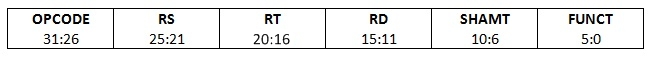
\includegraphics{r-format}
	\end{figure}
	
\begin{table}[H]
\centering	
\begin{tabular}{|c|l|}
	\hline 
	\cellcolor[gray]{0.9}\textbf{CAMPO} & \cellcolor[gray]{0.9}\textbf{DESCRIÇÃO} \\ 
	\hline 
	OPCODE & Código da operação básica da instrução. \\ 
	\hline 
	RS & Registrador do primeiro operando de origem. \\ 
	\hline 
	RT & Registrador do segundo operando de origem. \\ 
	\hline 
	RD & Registrador de destino. \\ 
	\hline 
	DON'T CARE & Não importa. \\ 
	\hline 
	FUNCT & Variante específica da operação. \\ 
	\hline 
	\end{tabular} 
	\end{table}	

\begin{table}[H]
\centering
	\begin{tabular}{|c|c|c|}
  	\hline 
  	\cellcolor[gray]{0.9}\textbf{OPCODE} & \cellcolor[gray]{0.9}\textbf{INSTRUCTION} & \cellcolor[gray]{0.9}\textbf{FUNCTION} \\ 
  	\hline 
  	0x00 & ADD & 0x20 \\ 
  	\hline 
  	0x00 & SUB & 0x22 \\ 
  	\hline 
  	0x1C & MUL & 0x02 \\ 
  	\hline 
  	0x05 & DIV & 0x01 \\ 
  	\hline 
  	0x00 & AND & 0x24 \\ 
  	\hline 
  	0x00 & OR & 0x25 \\ 
  	\hline 
  	0x00 & CMP & 0x2A \\ 
  	\hline 
  	0x00 & NOT & 0x27 \\ 
  	\hline
  	0x00 & NOP & 0x00 \\
  	\hline 
  	\end{tabular} 
  \end{table} 
  	 	
  	
	 Um segundo tipo de formato de instrução é chamado de formato I, utilizado pelas instruções imediatas e de transferência de dados.
	\begin{figure}[H]
    	\centering
    	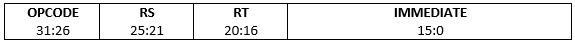
\includegraphics{i-format}
  	\end{figure}
  	
  	\begin{table}[H]
\centering	
\begin{tabular}{|c|l|}
	\hline 
	\cellcolor[gray]{0.9}\textbf{CAMPO} & \cellcolor[gray]{0.9}\textbf{DESCRIÇÃO} \\ 
	\hline 
	OPCODE & Código da operação básica da instrução. \\ 
	\hline 
	RS & Registrador do primeiro operando de origem. \\ 
	\hline 
	RT & Registrador de destino. \\ 
	\hline 
	IMMEDIATE & Constante numérica. \\ 
	\hline 
	\end{tabular} 
	\end{table}
	
\begin{table}[H]
\centering	
\begin{tabular}{|c|c|}
	\hline 
  	\cellcolor[gray]{0.9}\textbf{OPCODE} & \cellcolor[gray]{0.9}\textbf{INSTRUCTION} \\ 
	\hline 
	0x08 & ADDI \\ 
	\hline 
	0x09 & SUBI \\ 
	\hline 
	0x0C & ANDI \\ 
	\hline 
	0x0D & ORI \\ 
	\hline
	0x23 & LW \\ 
	\hline 
	0x2B & SW \\
	\hline
	0x04 & BRFL \\ 
  	\hline 
	\end{tabular} 
\end{table}	
	
 O formato Jump servem para as instruções de desvio incondicional.  	
   	\begin{figure}[H]
    	\centering
    	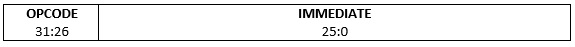
\includegraphics{jump}
		\label{jump}
  	\end{figure}
  	
\begin{table}[H]
\centering	
\begin{tabular}{|c|l|}
	\hline 
	\cellcolor[gray]{0.9}\textbf{CAMPO} & \cellcolor[gray]{0.9}\textbf{DESCRIÇÃO} \\ 
	\hline 
	OPCODE & Código da operação básica da instrução. \\ 
	\hline 
	IMMEDIATE & Constante numérica. \\ 
	\hline 
	\end{tabular} 
	\end{table}
 
\begin{table}[H]
\centering 	
  	\begin{tabular}{|c|c|}
  	\hline 
  	\cellcolor[gray]{0.9}\textbf{OPCODE} & \cellcolor[gray]{0.9}\textbf{INSTRUCTION} \\ 
  	\hline 
  	0x11 & JR \\ 
  	\hline 
  	0x02 & JPC \\ 
  	\hline 
  	0x03 & CALL \\ 
  	\hline 
  	0x01 & RET \\ 
  	\hline 
  	0x02 & HALT \\ 
  	\hline 
  	\end{tabular} 
\end{table}